\documentclass[tikz,border=12pt]{standalone}
\usepackage[T1]{fontenc}
\begin{document}
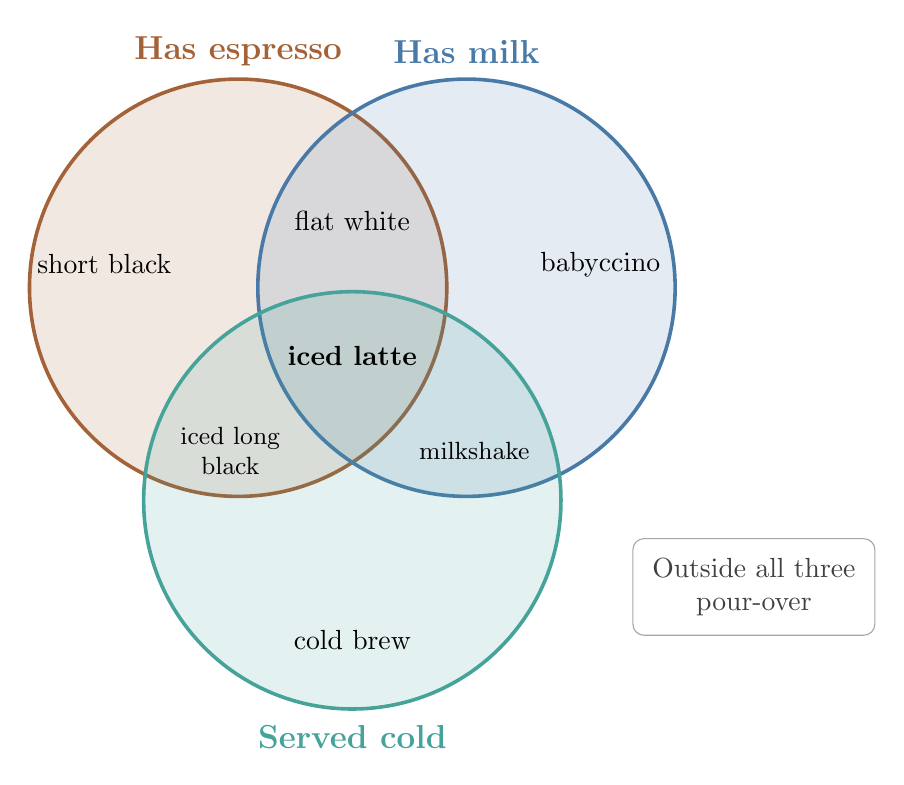
\begin{tikzpicture}[every node/.style={align=center}]
  % Three overlapping properties
  \definecolor{espresso}{HTML}{A36238}
  \definecolor{milk}{HTML}{4979A6}
  \definecolor{cold}{HTML}{46A39A}
  \filldraw[draw=espresso, line width=1.3pt, fill=espresso, fill opacity=.15] (-1.45,1.05) circle (2.65);
  \filldraw[draw=milk, line width=1.3pt, fill=milk, fill opacity=.15] (1.45,1.05) circle (2.65);
  \filldraw[draw=cold, line width=1.3pt, fill=cold, fill opacity=.15] (0,-1.65) circle (2.65);

  \node[font=\bfseries\large, text=espresso] at (-1.45,4.05) {Has espresso};
  \node[font=\bfseries\large, text=milk] at (1.45,4.05) {Has milk};
  \node[font=\bfseries\large, text=cold] at (0,-4.65) {Served cold};

  \node at (-3.15,1.35) {short black};
  \node at (3.15,1.35) {babyccino};
  \node at (0,1.9) {flat white};
  \node[font=\small] at (-1.55,-1.02) {iced long\\black};
  \node[font=\small] at (1.55,-1.02) {milkshake};
  \node[font=\bfseries] at (0,.18) {iced latte};
  \node at (0,-3.42) {cold brew};

  \node[draw=black!35, rounded corners=4pt, inner sep=7pt, text=black!75] at (5.1,-2.75) {Outside all three\\pour-over};
\end{tikzpicture}
\end{document}
